\documentclass{beamer}
\usetheme{Warsaw}

\usepackage{graphicx} % Allows including images
\usepackage{booktabs} % Allows the use of \toprule, \midrule and \bottomrule in tables
\usepackage{listings}
\usepackage[T1]{fontenc}
\usepackage[outline]{contour}
\usepackage[utf8]{inputenc}
\usepackage[overlay,absolute]{textpos}
\usepackage{tikz}
\usetikzlibrary{arrows,shapes}
\usepackage{amsfonts}


\AtBeginSection[]
{
\begin{frame}<beamer>
\frametitle{Plan}
\tableofcontents[
  currentsection,
  hideothersubsections
]
\end{frame}
}

\lstset{language=C++,
                basicstyle=\ttfamily,
                keywordstyle=\color{teal}\ttfamily,
                stringstyle=\color{red}\ttfamily,
                commentstyle=\color{cyan}\ttfamily,
                morecomment=[l][\color{magenta}]{\#},
                escapechar=@
}

\setbeamercolor{normal text}{fg=white,bg=black!90}
\setbeamercolor{structure}{fg=white}

\setbeamercolor{alerted text}{fg=red!85!black}

\setbeamercolor{item projected}{use=item,fg=black,bg=item.fg!35}

\setbeamercolor*{palette primary}{use=structure,fg=structure.fg}
\setbeamercolor*{palette secondary}{use=structure,fg=structure.fg!95!black}
\setbeamercolor*{palette tertiary}{use=structure,fg=structure.fg!90!black}
\setbeamercolor*{palette quaternary}{use=structure,fg=structure.fg!95!black,bg=black!80}

\setbeamercolor*{framesubtitle}{fg=white}

\setbeamercolor*{block title}{parent=structure,bg=black!60}
\setbeamercolor*{block body}{fg=black,bg=black!10}
\setbeamercolor*{block title alerted}{parent=alerted text,bg=black!15}
\setbeamercolor*{block title example}{parent=example text,bg=black!15}

\author[Félix-Antoine Ouellet]{Félix-Antoine Ouellet}
\title[Autovectorization\hspace{2em}\insertframenumber/\inserttotalframenumber]{Parallélisation automatique de boucles pour processeurs vectoriels}
\institute{Université de Sherbrooke}
\date{18 Septembre 2014}

\newcommand{\tikzmark}[1]{\tikz[remember picture] \node[coordinate] (#1) {#1};}

\begin{document}

\begin{frame}
\titlepage % Print the title page as the first slide
\end{frame}

\begin{frame}
\tableofcontents[hideallsubsections]
\end{frame}

\section{Motivation}
\subsection{Fin de la loi de Moore}
\begin{frame}
\frametitle{Loi de Moore}
\begin{center}
\begin{quote}
"Le nombre de transistors dans les microprocesseurs double tous les 18 mois."
\end{quote}
\end{center}
\hfill - Loi de Moore
\end{frame}

\begin{frame}
\frametitle{Constat de l'industrie}
\begin{center}
\begin{quote}
"The free lunch is over"
\end{quote}
\end{center}
\hfill - Herb Sutter
\end{frame}

\begin{frame}
\frametitle{Constat de l'industrie}
\begin{center}
\colorbox{white}{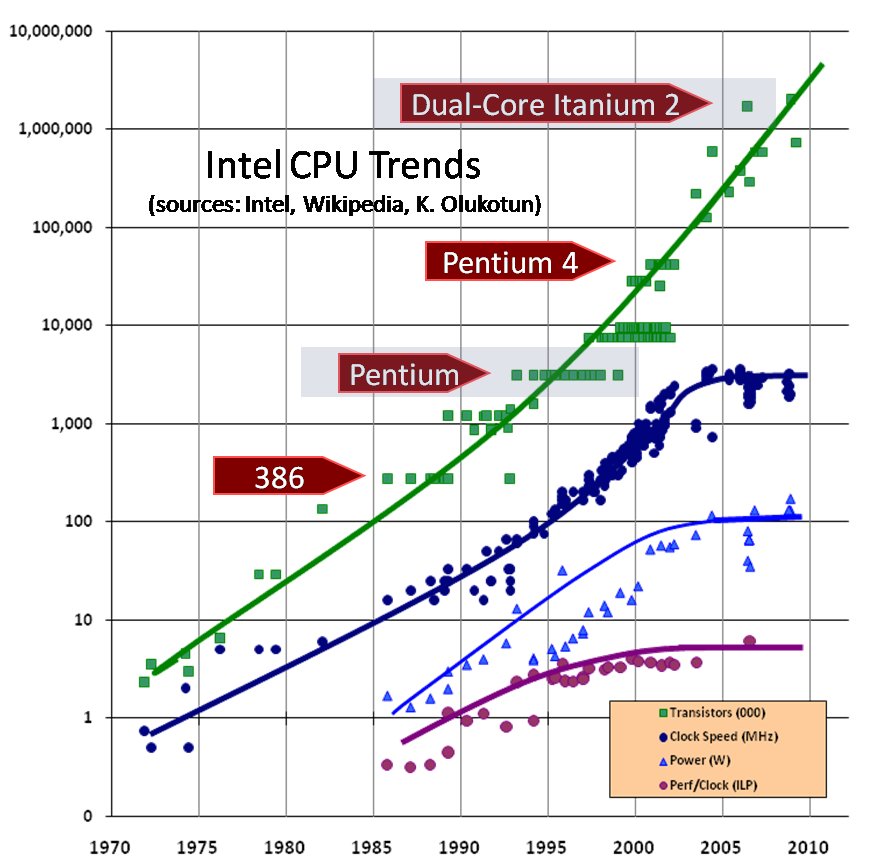
\includegraphics[scale=0.4]{CPU.png}}
\end{center}
\end{frame}

\subsection{Processeurs modernes}
\begin{frame}
\frametitle{Avenues possible}
\begin{itemize}
\item Processeurs multi-coeurs
\item Accélérateurs
\item Processeurs vectoriels
\end{itemize}
\end{frame}

\begin{frame}
\frametitle{Processeurs vectoriels}
\begin{center}
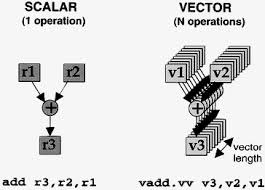
\includegraphics[scale=0.85]{Vector.jpg}
\end{center}
\end{frame}

\section{Exemple}
\begin{frame}[fragile]
\frametitle{Code Séquentiel}
\framesubtitle{Somme des éléments de vecteurs}
\begin{lstlisting}
int somme = 0;
for (int i = 0; i < 100; ++i) {
  somme += A[i];
}
\end{lstlisting}
\end{frame}

\begin{frame}[fragile]
\frametitle{Code Vectoriel}
\framesubtitle{Somme des éléments de vecteurs}
\begin{lstlisting}
int sommeTab[] = { 0, 0 };
for (int i = 0; i < 100; i+=8) {
  sommeTab[0] += A[i:i+3]; 
  sommeTab[1] += A[i+4:i+7];
}
int somme = 0;
for (int i = 0; i < 2; ++i) {
  somme += sommeTab[i];
}
for (int i = 96; i < 100; ++i) {
  somme += A[i];
}
\end{lstlisting}
\end{frame}

\section{Procédure}
\subsection{Notions de base}
\begin{frame}
\frametitle{Notions de base}
\framesubtitle{Dépendence mémoire}
Situation dans laquelle deux instructions accèdent à la même donnée.
\end{frame}

\begin{frame}[fragile]
\frametitle{Notions de base}
\framesubtitle{Classification des dépendences mémoire}
\begin{lstlisting}
void fct() {
  int a = 20;
  int b = a;
  /* ... */
  int c = d;
  int d = e;
}
\end{lstlisting}
\end{frame}

\begin{frame}[fragile]
\frametitle{Notions de base}
\framesubtitle{Classification des dépendences mémoire}
\begin{lstlisting}
void fct() {
  int @\textcolor{red}{a =}@ 20;
  int b @\textcolor{red}{= a};@
  /* ... */
  int c = d;
  int d = e;
}
\end{lstlisting}

\begin{textblock}{5}(8, 7)
	 \textcolor{red}{Vraie dépendence (Lecture après écriture)}
\end{textblock}
\end{frame}

\begin{frame}[fragile]
\frametitle{Notions de base}
\framesubtitle{Classification des dépendences mémoire}
\begin{lstlisting}
void fct() {
  int @\textcolor{red}{a =}@ 20;
  int b @\textcolor{red}{= a};@
  /* ... */
  int c @\textcolor{yellow}{= d}@;
  int @\textcolor{yellow}{d =}@ e;
}
\end{lstlisting}

\begin{textblock}{5}(8, 7)
	 \textcolor{red}{Vraie dépendence (Lecture après écriture)}
\end{textblock}

\begin{textblock}{5}(8, 10)
	\textcolor{yellow}{Anti-dépendence (Écriture après lecture)}
\end{textblock}
\end{frame}

\begin{frame}[fragile]
\frametitle{Notions de base}
\framesubtitle{Classification des dépendences de boucles}
\begin{lstlisting}
for (int i = 0; i < 100; ++i) {
  A[i] = B[i] + C[i];
  D[i] = A[i] + 10;
}

for (int i = 0; i < 100; ++i) {
  A[i+1] = A[i] + B[i];
}
\end{lstlisting}
\end{frame}

\begin{frame}[fragile]
\frametitle{Notions de base}
\framesubtitle{Classification des dépendences de boucles}
\begin{lstlisting}
for (int i = 0; i < 100; ++i) {
  @\textcolor{red}{A[i] =}@ B[i] + C[i];
  D[i] @\textcolor{red}{= A[i]}@ + 10;
}

for (int i = 0; i < 100; ++i) {
  A[i+1] = A[i] + B[i];
}
\end{lstlisting}

\begin{textblock}{5.5}(9, 7)
	\textcolor{red}{Dépendence indépendante de la boucle}
\end{textblock}
\end{frame}

\begin{frame}[fragile]
\frametitle{Notions de base}
\framesubtitle{Classification des dépendences de boucles}
\begin{lstlisting}
for (int i = 0; i < 100; ++i) {
  @\textcolor{red}{A[i] =}@ B[i] + C[i];
  D[i] @\textcolor{red}{= A[i]}@ + 10;
}

for (int i = 0; i < 100; ++i) {
  @\textcolor{yellow}{A[i+1] = A[i]}@ + B[i];
}
\end{lstlisting}

\begin{textblock}{5.5}(9, 7)
	\textcolor{red}{Dépendence indépendante de la boucle}
\end{textblock}

\begin{textblock}{5}(9, 11)
	\textcolor{yellow}{Dépendence portée par la boucle}
\end{textblock}
\end{frame}

\subsection{Analyse}
\begin{frame}[fragile]
\frametitle{Légalité}
\framesubtitle{Parallélisation des instructions}
\begin{lstlisting}
int somme = 0;
for (int i = 0; i < 100;
     ++i) {
  somme += A[i];
}
\end{lstlisting}

\begin{textblock}{6}(9, 6)
	\begin{itemize}
	\item<2->[\checkmark] Pas d'appels de fonctions
	\item<3->[\checkmark] Opération parallélisable
	\item<4->[\checkmark] Types des paramètres parallélisables
	\item<5->[\checkmark] Type de retour parallélisable
	\end{itemize}
\end{textblock}
\end{frame}

\begin{frame}[fragile]
\frametitle{Légalité}
\framesubtitle{Parallélisation de la mémoire}
\begin{lstlisting}
int somme = 0;
for (int i = 0; i < 100; ++i) {
  somme += A[i];
}
\end{lstlisting}

\begin{textblock}{6}(9, 10)
	\begin{itemize}
	\item<2->[\checkmark] Pas de chevauchement d'accès mémoire
	\item<3->[$\times$] Pas de dépendences mémoire
	\end{itemize}
\end{textblock}
\end{frame}

\begin{frame}
\frametitle{Profitabilité}
\begin{itemize}
\item Lié à l'architecture physique
\item Coût version séquentielle VS Coût version vectorielle
\end{itemize}

\begin{center}
\begin{tabular}{ | c | c | }
  \hline
  Séquentielle & Vectorielle \\
  \hline
  Coût add i64 & Coût add \textless2 x i64\textgreater \\
  \hline
  Coût load i64 & Coût load \textless2 x i64\textgreater \\
  \hline
\end{tabular}
\end{center}

\begin{itemize}
\item Meilleur facteur de déroulement
\end{itemize}
\end{frame}

\subsection{Transformations}
\begin{frame}
\frametitle{Reconnaissance d'idiomes}
\framesubtitle{Théorie}
\begin{itemize}
\item But: Agir en présence d'une situation connue
\item Exemples:
\begin{itemize}
\item Induction
\item Réduction
\end{itemize}
\end{itemize}
\end{frame}

\begin{frame}[fragile]
\frametitle{Reconnaissance d'idiomes}
\framesubtitle{Pratique}
\begin{lstlisting}
int somme = 0;
int sommeTab[2];
for (int i = 0; i < 2; ++i) {
  sommeTab[i] = 0;
  for (int j = i; j < 100; j+=2) {
    sommeTab[i] += A[j];
  }
  somme += sommeTab[i];
}
\end{lstlisting}
\end{frame}

\begin{frame}
\frametitle{Distribution de boucle}
\framesubtitle{Théorie}
\begin{itemize}
\item But: Regrouper les calculs similaires
\item Moyen: Produire plusieurs boucles à partir de la boucle originale
\end{itemize}
\end{frame}

\begin{frame}[fragile]
\frametitle{Distribution de boucle}
\framesubtitle{Pratique}
\begin{lstlisting}
int sommeTab[] = { 0, 0 };
for (int i = 0; i < 2; ++i) {
  for (int j = i; j < 100; j+=2) {
    sommeTab[i] += A[j];
  }
}
int somme = 0;
for (int i = 0; i < 2; ++i) {
  somme += sommeTab[i];
}
\end{lstlisting}
\end{frame}

\begin{frame}
\frametitle{Inter-échange de boucles}
\framesubtitle{Théorie}
\begin{itemize}
\item But: Optimiser les accès mémoire et exposer du parallélisme
\item Moyen : Échanger les variables d'induction des boucles ciblées
\end{itemize}
\end{frame}

\begin{frame}[fragile]
\frametitle{Inter-échange de boucles}
\framesubtitle{Pratique}
\begin{lstlisting}
int sommeTab[] = { 0, 0 };
for (int j = 0; j < 100; j+=2) {
  for (int i = j; i < min(j+2, 100); ++i) {
     sommeTab[i-j] += A[j+i];
  }
}
int somme = 0;
for (int i = 0; i < 2; ++i) {
  somme += sommeTab[i];
}
\end{lstlisting}
\end{frame}

\begin{frame}
\frametitle{Vectorization}
\framesubtitle{Théorie}
\begin{itemize}
\item But: Exploiter les registres et opérations vectoriels disponibles
\item Moyen : Générer du code vectoriel
\end{itemize}
\end{frame}

\begin{frame}[fragile]
\frametitle{Vectorization}
\framesubtitle{Pratique}
\begin{lstlisting}
int sommeTab[] = { 0, 0 };
for (int j = 0; j < 100; j+=4) {
  for (int i = j; i < min(j+2, 100); ++i) {
    sommeTab[i-j] += A[j:j+3];
  }
}
int somme = 0;
for (int i = 0; i < 2; ++i) {
  somme += sommeTab[i];
}
\end{lstlisting}
\end{frame}

\begin{frame}
\frametitle{Déroulage de boucle}
\framesubtitle{Théorie}
\begin{itemize}
\item But: Réduire le temps d'exécution d'une boucle
\item Moyen : Expliciter les calculs dans une boucle
\item Attention, on choisit de prendre plus de mémoire pour gagner en vitesse d'exécution
\end{itemize}
\end{frame}

\begin{frame}[fragile]
\frametitle{Déroulage de boucle}
\framesubtitle{Pratique}
\begin{lstlisting}
int sommeTab[] = { 0, 0 };
for (int i = 0; i < 100; i+=8) {
  sommeTab[0] += A[i:i+3]; 
  sommeTab[1] += A[i+4:i+7];
}
int somme = 0;
for (int i = 0; i < 2; ++i) {
  somme += sommeTab[i];
}
for (int i = 96; i < 100; ++i) {
  somme += A[i];
}
\end{lstlisting}
\end{frame}

\section{Problèmes ouverts}

\begin{frame}[fragile]
\frametitle{Pointeurs}
\begin{lstlisting}
void bar(float *A, float *B, float K, int n) {
  for (int i = 0; i < n; ++i)
    A[i] *= B[i] + K;
}
\end{lstlisting}
\end{frame}

\begin{frame}[fragile]
\frametitle{\textit{Superword Level Parallelism}}
\begin{lstlisting}
void foo(int a1, int a2, 
         int b1, int b2, int *A) {
  A[0] = a1*(a1 + b1)/b1 + 50*b1/a1;
  A[1] = a2*(a2 + b2)/b2 + 50*b2/a2;
}
\end{lstlisting}
\end{frame}

\section{Conclusion}
\begin{frame}
\frametitle{Conclusion}
\begin{itemize}
\item Trois grandes étapes
\item<2-> L'autovectorization c'est bien, mais c'est limité
\item<3-> L'architecture change donc la programmation doit changer
\end{itemize}
\end{frame}

\end{document}